\documentclass[pdf, aspectratio=169]{beamer}
\usepackage[]{hyperref,graphicx,siunitx,lmodern,booktabs,tikz,tensor}
\usepackage{pgfplots,pgfplotstable}
\usepackage{pdfpc-commands}

\usepackage[mode=buildnew]{standalone}
\mode<presentation>{\usetheme{Astro}}

\graphicspath{ {../Images/} }

\sisetup{per-mode=symbol}
\usetikzlibrary{calc,intersections, decorations.pathmorphing,shadings}
%\tikzstyle{proton}=[circle, minimum size = 7mm, ball color=red, black,transform shape]
%\tikzstyle{neutron}=[circle, minimum size=7mm, ball color=gray, black, transform shape]
%\tikzstyle{gammaray}=[ultra thick, -latex, decorate, decoration={snake, post length=3mm}]


%preamble
\title{What happens in the event horizon\ldots}
\date{November 12, 2018}
\author{Jed Rembold}

\begin{document}
\renewcommand*{\theenumi}{\Alph{enumi}}

\begin{frame}{Announcements}
  \begin{itemize}
	\item Webwork due on Wednesday
	\item Test 3 on Friday!
	  \begin{itemize}
		\item Review questions, old test, and all accompanying solutions posted
		\item Equation sheet also updated
		\item Covers Lectures 21--30
			\begin{itemize}
				\item Corresponds to Chapter 15-24 (minus Ch 20)
			\end{itemize}
		\item Email me if you need to borrow a calculator!
	  \end{itemize}
	\item Polling: \url{rembold-class.ddns.net}
  \end{itemize}
\end{frame}

\begin{frame}{APOD!}
	\begin{center}
		\includegraphics[width=.7\textwidth]{APOD_LagoonNebula.jpg}
	\end{center}
\end{frame}

\begin{frame}{Review Question}
  What happens as a white dwarf star gains enough mass to equal the Chandrasakhar Limit?
  \begin{enumerate}
	\item \alert<2>{Carbon fusion ignites in the star, causing a supernova}
	\item Hydrogen fusion ignites in a shell around the star, causing a small nova
	\item The star collapses into a neutron star, giving off a tremendous amount of energy in the process
	\item Rotational forces rip the star apart, scattering its gases
  \end{enumerate}
\end{frame}

\begin{frame}{Structure of a Pulsar}
  \begin{columns}
	\column{.5\textwidth}
	\begin{itemize}
	  \item Strong magnetic fields focus outgoing radiation
	  \item Results in a ``lighthouse'' effect
	  \item Spins very fast due to conservation of angular momentum
	  \item Rapid spinning causes these beams of radiation to sweep across us
	\end{itemize}
	\column{.5\textwidth}
	\begin{center}
	  \includegraphics[width=.9\textwidth]{ch14_pulsar.jpg}
	\end{center}
  \end{columns}
\end{frame}

\fullFrameMovie{../Videos/Pulsar.ogv}{../Videos/Pulsar.png}

\begin{frame}{Tick Tock}
  \begin{itemize}
	\item Isolated pulsars will eventually slow as they lose angular momentum and energy to the outgoing gases
	\item Pulsars as part of binary systems may actually speed up
	  \begin{itemize}
		\item A steady diet of more mass lends more angular momentum
		\item Can end up pulsing every few thousandths of a second
	  \end{itemize}
	\item There is a rotational speed limit
	  \begin{itemize}
		\item If you spin too fast, gravity can't keep everything contained
		\item Is what tells us pulsars must be neutron stars and not white dwarfs
	  \end{itemize}
  \end{itemize}
\end{frame}

\begin{frame}{Magnetars}
  \begin{columns}
	\column{.5\textwidth}
	\begin{itemize}
	  \item When spin, temperature, and magnetic field combine in the right combination
	  \item Magnifies magnetic field: creates a dynamo
	  \item Magnetic fields up to $10^{11}$ teslas
		\begin{itemize}
		  \item Earth magnetic field: \SI{5e-5}{\tesla}
		  \item We can't create more than maybe 100-1000 T without ripping apart our machines
		\end{itemize}
	  \item 1 in 10 supernova could create?
	\end{itemize}
	\column{.5\textwidth}
	\begin{center}
	  \includegraphics[width=.9\textwidth]{ch14_magnetar.jpg}
	\end{center}
  \end{columns}
\end{frame}

\begin{frame}{The Power of the (Magnetic) Force}
  \begin{columns}
	\column{.7\textwidth}
	\begin{itemize}
	  \item Magnetic fields create forces on moving charges
		\begin{itemize}
		  \item Say, for instance, the protons and electrons in atoms
		\end{itemize}
	  \item Getting a moon distance away would wipe all your credit cards
	  \item Getting within several thousand kilometers would render all your biochemistry useless
	  \item Getting within 1000 kilometers and your molecular structure just kinda\ldots dissolves!
	\end{itemize}
	\column{.3\textwidth}
	\begin{center}
	  \includegraphics[width=.5\textwidth]{ch14_dissolve_man.pdf}
	\end{center}
  \end{columns}
\end{frame}

\begin{frame}{Starquakes}
  \begin{itemize}
	\item Crust of magnetar and the magnetic field are locked together
	  \begin{itemize}
		\item Changing one changes the other\ldots
	  \end{itemize}
	\item Crust is under huge pressure from gravity, rotation, and the magnetic field
	\item A tiny slip, even just a centimeter, releases an insane amount of energy
	  \begin{itemize}
		\item Force the magnetic field to ``slip'' as well
		\item Equivalent to a solar flare, just far, far, far more energetic
	  \end{itemize}
	\item Swift: 2004
	  \begin{itemize}
		\item Designed to look at high energy x-ray sources
		\item Wasn't even looking in the direction of the magnetar flare
		\item The amount of radiation swamped and oversaturated all its sensors
		\item Compressed the Earth's magnetic field and ionized upper atmosphere
		\item All from 50,000 light-years away\ldots
	  \end{itemize}
	\item Thankfully, these are rare
  \end{itemize}
\end{frame}

\begin{frame}{Grave \#3}
	\begin{center}
		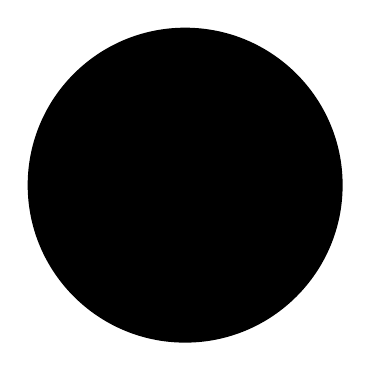
\begin{tikzpicture}
			\fill[black] (0,0) circle (2);
		\end{tikzpicture}
	\end{center}
\end{frame}

\begin{frame}{The Great Escape}
  \begin{itemize}
	\item Let's talk the speed required to escape an gravitational mass
	\item Should depend on the mass of the object and our initial distance away from it
	\item If we want to barely escape, then we need our final velocity to be 0
	\item<2> This requires that:
	  \begin{block}{Escape Speed}
		\[v = \sqrt{\frac{2GM}{R}}\]
	  \end{block}
  \end{itemize}
\end{frame}

\begin{frame}{Making the Escape}
  \begin{center}
	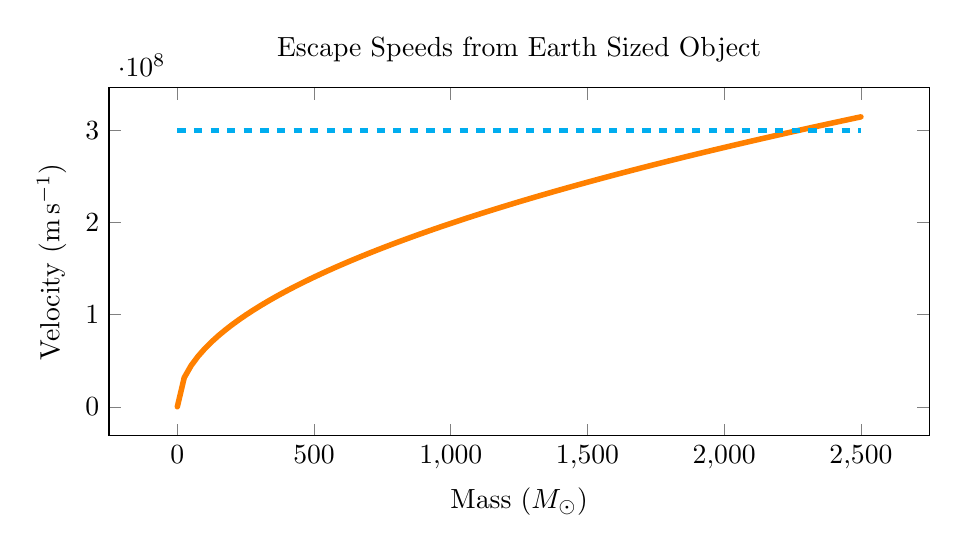
\begin{tikzpicture}
	  \begin{axis}[
		  xlabel = Mass ($M_\odot$),
		  ylabel = Velocity (\si{\meter\per\second}),
		  ylabel near ticks,
		  height=6cm,
		  width=12cm,
		  title=Escape Speeds from Earth Sized Object,
		]
		\addplot[domain=0:2500, samples=100, orange, line width=2pt, line cap=round] {sqrt(2*6.67e-11*2e30*x/6730000)};
		\draw<2>[ultra thick, cyan, dashed] (axis cs: 0,3e8) -- (axis cs: 2500,3e8);
	  \end{axis}
	\end{tikzpicture}
  \end{center}
\end{frame}

\begin{frame}{The Point of No Escape}
  \begin{itemize}
	\item Since nothing can go faster than light, for any mass there exists a radius from whence nothing could escape!
	\item Rewriting our escape velocity:
	  \begin{align*}
		c^2 &= \frac{2GM}{R} \\
		R &= \frac{2GM}{c^2}
	  \end{align*}
	\item This radius is called the Schwarzchild radius
	\item Even light couldn't escape from within this radius
	\item Makes it ``Black''
	\item And thus we have a theoretical ``Black Hole''
	\item In actuality, created when collapsing stars mass great enough to overcome neutron degeneracy
  \end{itemize}
\end{frame}

\begin{frame}{Some Examples}
  \begin{example}
	What is the Schwarzchild radius for our Sun? ($M_\odot = \SI{2e30}{\kilo\gram}$)
	\onslide<2->{
	\[R = \frac{2(\num{6.67e-11})(\num{2e30})}{(\num{3e8})^2} = \SI{2964}{\meter}\]
  }
  \end{example}
  \begin{example}
	What is the Schwarzchild radius of YOU? ($M = \SI{70}{\kilo\gram}$)
	\onslide<3>{
	  \[R = \frac{2(\num{6.67e-11})(70)}{(\num{3e8})^2} = \SI{1e-25}{\meter}\]
  }
  \end{example}
\end{frame}

\begin{frame}{The Event Horizon}
  \begin{columns}
	\column{.25\textwidth}
	\begin{center}
	  \vspace{-8mm}
	  \begin{tikzpicture}[scale=1, transform shape]
		\coordinate (center) at (0,-.1);
		\clip[rounded corners] ($(center)-(2,2)$) rectangle ($(center)+(2,2)$);
		\node[inner sep=0pt, outer sep=0pt] at (0,0) {\includegraphics[width=8cm]{ch14_event_horizon.jpg}};
	  \end{tikzpicture}
	\end{center}
	\column{.6\textwidth}
	  \begin{itemize}
		\item Since no light can escape, it is impossible for us to see any events that happen within the Schwarzchild radius
		\item It is as if they were ``beyond the horizon''
		\item Another name for the Schwarzchild radius is the \alert{Event Horizon}
		\item Both describe the point at which light can no longer escape
		\item Commonly imagined as the ``edge'' of the black hole
	  \end{itemize}
  \end{columns}
\end{frame}

\begin{frame}{Understanding Check}
  You know that the event horizon of a particular black hole has a radius of \SI{30}{\kilo\meter}. How massive is the black hole (in solar masses)? ($G=\num{6.67e-11}, M_\odot = \num{2e30}, c=\num{3e8}$)

  \begin{enumerate}
	\item $(\num{3.4e-8}) M_\odot$
	\item $0.01M_\odot$
	\item \alert<2>{$10M_\odot$}
	\item $(\num{2e31}) M_\odot$
  \end{enumerate}
\end{frame}

\begin{frame}{Misconceptions}
  \begin{itemize}
	\item Our Sun may one day turn into a black hole
	  \begin{itemize}
		\item<2-> Utterly, utterly false. Our Sun has nowhere near the mass needed to push past both the electron and neutron degeneracy pressures to form a black hole.
	  \end{itemize}
	\item Black Holes are the universe's vaccuum cleaners, sucking in all their surroundings
	  \begin{itemize}
		\item<3-> Nope! Black holes have a lot of mass and gravity, but if you are far away that's all you see. We could happily keep orbiting the Sun even if it were to pop into a black hole this instant!
	  \end{itemize}
  \end{itemize}
\end{frame}

\begin{frame}{Big Fish, Small Fish}
  \begin{itemize}
	\item Stellar Mass Black Holes
	  \begin{itemize}
		\item Generally several solar masses to a dozen or so
		\item Results in fairly small event horizons
	  \end{itemize}
	\item Supermassive Black Holes
	  \begin{itemize}
		\item Many times larger than the Sun
		\item Anchor the center of many galaxies
		\item The one at the center of the Milky Way is estimated at 4,300,000$M_\odot$!!
		\item May actually be crucial to galaxy formation
	  \end{itemize}
  \end{itemize}
\end{frame}

\begin{frame}{A Poor Decision}
  \begin{center}
	So what happens as you fall into a black hole?\vspace{1cm}

  \pause
	\textcolor{Red}{\Huge YOU DIE!}
  \pause

  \vspace{1cm}
  But what about in the meanwhile? What would happen?
  \end{center}
\end{frame}

\begin{frame}{Tidal Spaghetti}
  \begin{itemize}
	\item Recall that the gravity of Jupiter exerts tidal forces on Io
	  \begin{itemize}
		\item Squeeze and stretch the moon
	  \end{itemize}
	\item Black holes have MUCH more gravity
	  \begin{itemize}
		\item And thus MUCH stronger tidal forces!
	  \end{itemize}
	\item Your feet would feel a force thousands of times more than your head!
	  \begin{itemize}
		\item Get stretched!
	  \end{itemize}
	\item Process known as:\vspace{5mm}
	  \begin{center}
		\onslide<2>{\textcolor{cyan}{\Huge Spaghettification!}
		\includegraphics[width=.4\textwidth]{ch14_spaghetti.jpg}}
	  \end{center}
  \end{itemize}
\end{frame}

\begin{frame}{Space-Time}
  \begin{itemize}
	\item Einstein showed that space and time are both related
	\item Can envision as a two dimensional rubber sheet
	\item Large masses cause indentations in the sheet and bend the trajectories of objects near them
	\item Since space and time are related, the more space you cross, the slower time ticks
  \end{itemize}
  \begin{center}
	\includegraphics[width=.8\textwidth]{ch14_spacetime.jpg}
  \end{center}
\end{frame}

\begin{frame}{Time Drags}
  \begin{itemize}
	\item As you approach a black hole, the curvature of space-time becomes extreme
	\item \alert{As viewed from the outside} your time slows down!
	  \begin{itemize}
		\item Can also envision as the light emitted each second takes longer and longer to reach the observer.
		\item YOUR time, as far as you are concerned, does not change
	  \end{itemize}
	\item Outsider observer never sees someone cross the event horizon
	\item The traveler sees the opposite
	  \begin{itemize}
		\item Looking outward, time appears accelerated
		\item Would see the entire future of the universe before crossing the event horizon
	  \end{itemize}
  \end{itemize}
\end{frame}

%\begin{frame}{Portals across the Universe}
  %\begin{itemize}
	%\item Supermassive black holes actually have weaker tidal forces
	  %\begin{itemize}
		%\item Their size means you need to be further away from the singularity
	  %\end{itemize}
	%\item Could maybe cross without being spaghettified
	%\item Rotating or charged black holes have bizarre properties
	%\item Wormholes to other dimensions?
  %\end{itemize}
%\end{frame}

%\begin{frame}{How do we find them?}

  %\begin{itemize}
	%\item Noting their orbital effects
	  %\begin{itemize}
		%\item Their huge mass makes an obvious effect on their surroundings
		%\item Look for everything orbiting something that can't be seen!
	  %\end{itemize}
	%\item Gravitational Lensing
	  %\begin{itemize}
		%\item Light can be bent as it passes the black hole
	  %\end{itemize}
  %\end{itemize}
  %\begin{center}
	%\includegraphics[width=.5\textwidth]{ch14_grav_lensing.jpg}
  %\end{center}
%\end{frame}

%\begin{frame}{LIGO!}
	%\begin{itemize}
		%\item Can now use gravity waves to look for energetic events from black holes!
			%\begin{itemize}
				%\item Swallowing of neutron star by black hole
				%\item Merging of two black holes
			%\end{itemize}
		%\item Stretches are TINY!
			%\begin{itemize}
				%\item Like measuring differences in a human hair from here in Alpha Centauri!
			%\end{itemize}
		%\item Earth stretches and squeezes as the wave moves past us
	%\end{itemize}
%\end{frame}



\end{document}
